\chapter{Brukergrensesnitt og brukersentrert utvikling} \label{chap:bakgrunn}
Dette kapittelet presenterer bakgrunnsteori om brukergrensesnitt og brukersentrert utvikling. 

\section{Brukergrensesnitt}

I dette delkapittelet presenteres brukbarhet, universell utforming og dialogprinsipper for interaktive systemer. Dette er viktig konsepter for å oppnå gode brukergrensesnitt. 

\subsection{Brukbarhet}
I \acrshort{iso} 9241-11 \citep{ISO9241-11} er brukbarhet definert som anvendbarhet, effektivitet og tilfredsstillelse for bestemte brukere med bestemte mål i bestemte omgivelser.
\begin{itemize}
\item Anvendbarhet er i hvilken grad brukeren klarer å utføre forhåndsdefinerte oppgaver, og oppnå forhåndsdefinerte mål.
\item Effektivitet er hvor effektiv brukeren er til å utføre forhåndsdefinerte oppgaver.
\item Tilfredsstillelse er brukerens opplevelse av systemet, den opplevde brukskvaliteten.
\end{itemize}

Anvendbarheten, effektiviteten og tilfredsstillelsen kan ikke evalueres isolert. Det må måles for de brukerne som er ment å bruke systemet, for de oppgavene systemet er ment å løse og i de omgivelsene systemet er ment i. 

Anvendbarhet og effektivitet kan enkelt måles ved telling. Anvendbarheten måles ved at man regner ut hvor mange prosent av de forhåndsdefinerte oppgavene brukeren klarte å utføre. Effektivitet kan måles ved å ta tiden på utføring av forhåndsdefinerte oppgaver.

Tilfredsstillelse er vanskeligere å måle. Standardiserte spørreskjema kan benyttes, men følelser er generelt vanskelig å representere i et spørreskjema.

\subsection{Universell utforming}
En utfordring ved utvikling av grensesnitt er at folk er forskjellige når det kommer til motivasjon, evner, bakgrunn, personlighet, alder og kjønn. Målet med universell utforming er å utvikle grensesnitt som ivaretar behovene til alle brukere.

Ved utvikling av universelt design bør man passe på å ikke lage et “minste felles multiplum” eller en “fordumming” av systemet som gjør det mindre nyttig for mange brukere \citep{MMIboken25}. Det er viktig å legge til rette for bruk av dårlig teknologi \footnote{Dårlig teknologi: for eksempel må det legges til rette for å kunne bruke gamle/trege datamaskiner}, brukere med lite teknisk erfaring og brukere med funksjonshemninger. Man må imidlertid også påse at systemet fungerer bra for andre brukere.

Ved utvikling av grensesnittet til et system som er laget for pasienter som tar flere legemidler fast bør det tas spesielle hensyn, blant annet fordi denne brukergruppen består av mange eldre. Når folk blir eldre skjer det forandringer i deres funksjonelle ferdigheter. Oppfattelsesevne, responshastighet og kognitive evner reduseres. Det er individuelle forskjeller i hvor fort disse forandringene skjer \citep{designForGamlisser}. 

Brukergrensesnitt kan bli mer brukervennlig for eldre dersom brukerne får kontroll over fontstørrelse, fargekontraster og lydvolum. Bedre pekeenheter, tydeligere navigasjonsstier og konsekvent layout kan også bidra til at brukergrensesnitt blir mer brukervennlig. Selv om disse forbedringene gjør størst forskjell for eldre, vil de øke brukervennligheten for andre aldersgrupper \citep{designForGamlisser}.

I Norge stilles det krav om universell utforming av \acrshort{ikt}-løsninger ved lov, jf diskriminerings- og tilgjengelighetsloven §14. Loven blir presisert i forskrift om universell utforming av \acrshort{ikt}-løsninger §2 og §4\footnote{Informasjon og veiledning for forskrift om universell utforming: \url{http://uu.difi.no/}}, der kommer det frem at man må følge \acrshort{wcag} (2.0)-standarden når man lager nettsider som retter seg mot “allmennheten”. 

\subsubsection{WCAG 2.0}
\acrfull{wcag} 2.0 er en del av en serie med retningslinjer for å gjøre internett tilgjengelig for alle, uavhengig av hvilke verktøy som brukes får å navigere på nettet, eller hvilke begrensninger brukere opererer under. 

\acrshort{wcag} 2.0 er bygd opp av fire prinsipper, som er videre inndelt i 12 retningslinjer og 61 testbare suksesskriterier. Suksesskriteriene er inndelt i tre nivåer: A, AA og AAA. Oppbyggingen er illustrert i figur~\ref{fig:wcag_tabell}.

\begin{figure}[H]
    \centering
    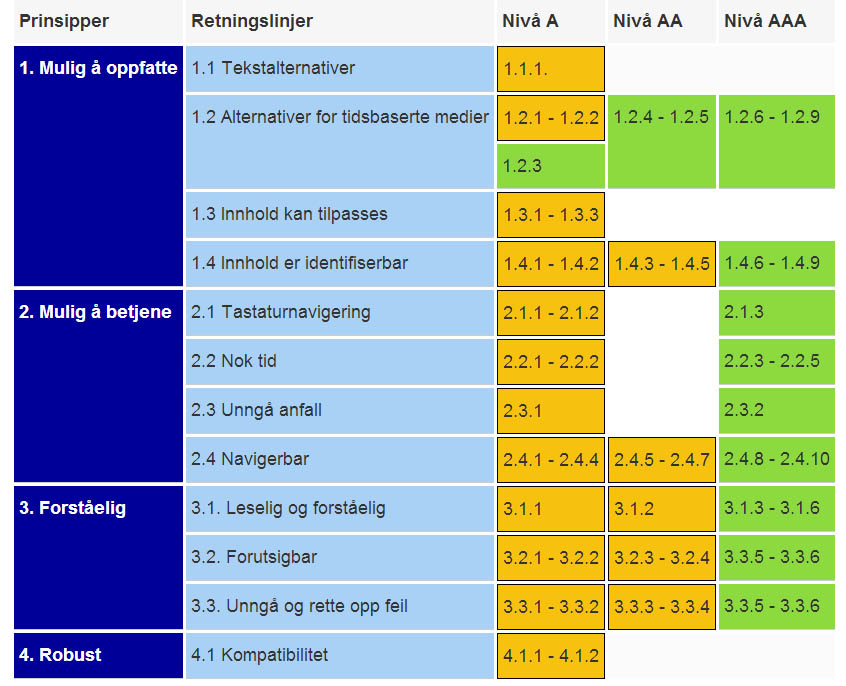
\includegraphics[width=0.9\textwidth]{fig/bakgrunn/wcag_tabell.jpg}
    \caption{Oppbygging av \acrshort{wcag} 2.0. De oransje kravene er omfattet av forskrift for universell utforming av \acrshort{ikt}-løsninger. Kilde: \url{http://uu.difi.no/veiledning/nettsider/krav-til-nettsider/oppbygging-av-wcag-20} }
    \label{fig:wcag_tabell}
\end{figure}

Forskrift om universell utforming av \acrshort{ikt}-løsninger fastslår at tilgjengelige nettsider skal lages i samsvar med nivåene A og AA, med unntak av kravene som gjelder teksting av direktesendt lyd og synstolking av innspilt video. Forskriften stiller dermed krav om at 35 av de 61 suksesskriterier skal følges.

\subsection{Dialogprinsipper}
\acrshort{iso} 9241-110:2006 "Ergonomi for samhandling mellom menneske og system - Del 110: Dialogprinsipper" beskriver 7 dialogprinsipper for interaktive systemer. En dialog defineres som en interaksjon mellom en bruker og et interaktivt system i form av brukerhandlinger og systemsvar som skal til for å oppnå et mål. Dialogprinsippene gjelder utformingen av brukergrensesnitt og skal bidra til å økt brukervennlighet for interaktive systemer. 


\section{Brukersentrert utvikling} \label{sec:brukersentrert}
Brukersentrert utvikling er en utviklingsfilosofi som handler om aktiv involvering av brukere gjennom hele utviklingsprosessen. Brukerdrevet utvikling fokuserer på å oppnå høy brukbarhet, og er mye brukt i systemutvikling. 

\acrshort{iso} 9241-210:2010 “Ergonomi for samhandling mellom menneske og system - Del 210: Menneskeorientert design for interaktive systemer” beskriver fire brukersentrerte aktiviteter som bør finne sted i brukersentrert utvikling:
\begin{enumerate}
\item Forstå og spesifisere brukskonteksten
\item Spesifisere brukernes og organisasjonens krav
\item Utvikle designløsninger
\item Evaluere design mot krav
\end{enumerate}

\begin{figure}[H]
    \centering
    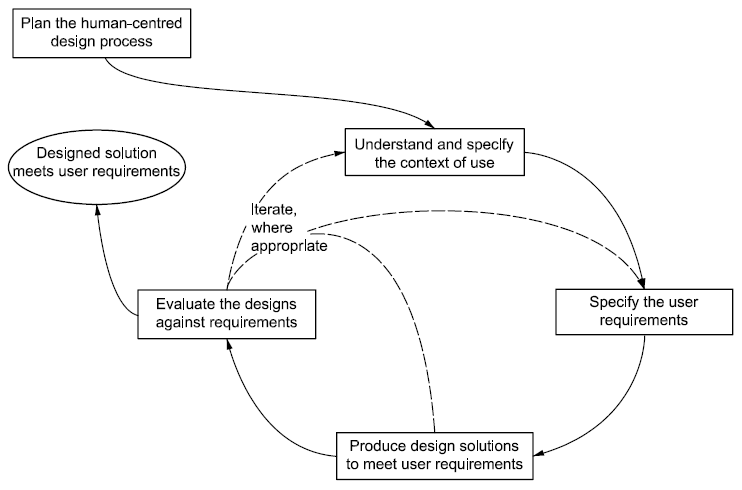
\includegraphics[width=0.8\textwidth]{fig/bakgrunn/ISO9241-210.PNG}
    \caption{Den gjensidige avhengigheten i brukersentrerte designaktiviteter, kilde: ISO 9241-210:2010 }
    \label{fig:ISO9241}
\end{figure}

Utviklingsaktivitetene inngår i en iterativ prosess der hver aktivitet kan bruke resultatene fra en annen aktivitet. Aktivitetene utføres ikke i streng rekkefølge. Standarden erkjenner at i det virkelige liv må man noen ganger gå tilbake til tidligere aktiviteter, og revurdere hva som gjøres der, etter å ha utført en aktivitet. Ulike aktiviteter kan skje samtidig. Prosessen er illustrert i figur~\ref{fig:ISO9241}.

Brukerdrevet utvikling kan være kostbart i form av at det er tidkrevende, men vil kunne være kostnadsbesparende på sikt ved at brukernes behov blir kartlagt underveis i utviklingsprosessen. Involvering av brukere i utviklingsprosessen er en verdifull kilde til informasjon om brukskontekst og oppgavene systemet skal løse \citep{usercentereddesign}.


\section{Prototyping} \label{sec:prototyping}
Prototyping er mye brukt i brukersentrert utvikling. Prototyping er prosessen som benyttes for å lage prototyper av systemer. En prototype er en foreløpig utgave av et system som lages før selve systemet settes i produksjon. Prototyper brukes til å demonstrere konsepter, teste designmuligheter og få innsikt i problemer og mulige løsninger \citep{suBoken}.

\begin{figure}[H]
    \centering
    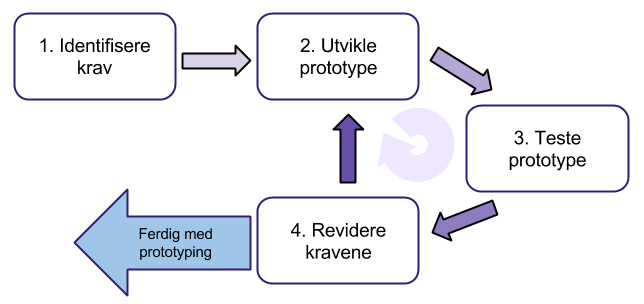
\includegraphics[width=1\textwidth]{fig/bakgrunn/prototype.png}
    \caption{Trinnene i prototypingsprosessen}
    \label{fig:prototype}
\end{figure}

Figur~\ref{fig:prototype} illustrerer prototypingsprosessen. Prosessen består av en rekke trinn som gjennomføres iterativt, der resultatet av en prototypetest danner grunnlaget når en ny prototype utvikles:
\begin{enumerate}
\item \textbf{Identifisere krav:} I det første trinnet identifiseres initielle krav og spesifikasjonene for systemet.
\item \textbf{Utvikle Prototype:} En prototype blir utviklet basert på kravene og spesifikasjonene som er identifisert.
\item \textbf{Teste prototype:} Den ferdige prototypen evalueres gjennom en prototypetest med brukere.
\item \textbf{Revidere kravene:} Kravene og spesifikasjonene for systemet blir revidert basert på tilbakemeldingene som er mottatt i prototypetesten. Hvis prototypeprosessen ikke er avsluttet etter dette trinnet, blir trinn 2-4 gjentatt. En ny prototype blir da utviklet, enten fra bunnen av eller som en forbedret versjon av den gamle prototypen.
\end{enumerate}

Før en prototype utvikles blir det tatt beslutninger om hvilken funksjonelle krav som skal inkluderes. For å minimere tiden det tar å lage prototypen er det bare den viktigste funksjonaliteten som blir inkludert\citep{suBoken}. En prototype er en forenklet versjon av det endelige systemet. Ved å teste et endelig system kan man få bedre tilbakemeldinger, men det er mer krevende. Prototyping gjør det mulig å få verdifulle tilbakemeldinger tidlig i utviklingsprosessen. Når endringer i kravspesifikasjon eller design oppdages tidlig krever det mindre arbeid å implementere endringene.

Det finnes mange typer prototyper, for eksempel papirbaserte prototyper og klikkbare digitale prototyper. Papirbaserte prototyper er skisser av et system, laget for hånd eller ved hjelp av digitale verktøy. Papirversjoner av elektroniske systemer kan være vanskelig å forstå for brukere, noe som kan føre til at tilbakemeldingene ved testing av funksjonalitet blir mindre verdifulle. 
En klikkbar digital prototype ligner mer på et ferdig system enn en papirprototype, da noe brukerinteraksjon er mulig ved hjelp av museklikk og tastetrykk. 

Papirbaserte prototyper har den fordel at de er raske og enkle å lage. Ifølge \citep{prototypingWebDesign} har papirprototyper også en fordel ved at brukere er mer komfortabel med å komme med tilbakemeldinger og kritikk av papirprototyper enn digitale prototyper. De begrunner dette med at papirprototyper virker mindre ``ferdig'' og ``ekte'' enn digitale prototyper, og at det fremstår som mindre arbeidskrevende å implementere foreslåtte endringer.



